% no answer key
% \documentclass[letterpaper]{exam}

% answer key
\documentclass[letterpaper, landscape]{exam}
\usepackage{2in1, lscape} 
\printanswers

\usepackage{units} 
\usepackage{xfrac} 
\usepackage[fleqn]{amsmath}
\usepackage{float}
\usepackage{mdwlist}
\usepackage{booktabs}
\usepackage{cancel}
\usepackage{polynom}
\usepackage{caption}
\usepackage{fullpage}
\usepackage{comment}
\usepackage{enumerate}
\usepackage{graphicx}

\usepackage{mathtools} 

\newcommand{\dg}{\ensuremath{^\circ}} 
\newcommand{\sgn}{\operatorname{sgn}}

\everymath{\displaystyle}
\title{Calculus I \\ Homework Fourteen \\ Sections 3.7 and 3.9}
\author{}
\date{\today}

\begin{document}

  \maketitle

  \section{Homework}
    \begin{itemize*}
      \item section 3.7: 7, 9-11, 15, 18, 23, 24 
      \item section 3.9: 1-6, 14, 18, 21, 24
    \end{itemize*}

  \ifprintanswers

  \section{Solutions}

  \subsection{Section 3.7}

  \begin{description}
    % \item[5] 
    %   \begin{enumerate}[(a)]
    %     \item The particle is speeding up between 0 and 1 seconds and slowing down after 
    %       $t = \unit[1]{s}$.

    %     \item The particle is slowing down between 0 and 1 seconds and after 2 seconds and speeding
    %       up between 1 and 2 seconds.

    %   \end{enumerate}

    % \newpage

    % \item[6] 
    %   \begin{enumerate}[(a)]
    %     \item The particle is slowing down between 0 and 2 seconds and speeding up after 
    %       $t = \unit[2]{s}$.

    %     \item The particle is traveling at a roughly constant velocity between 0 and 2 seconds and
    %       speeding up after that.

    %   \end{enumerate}

    \item[7]
      \begin{enumerate}[(a)]
        \item 
          \begin{align*}
            v(t)          & = 3t^2 - 9t - 7 \\
            \\
            3t^2 - 9t - 7 & = 0 \\
            t             & = \boxed{ \unit[4]{s} } \\
          \end{align*}

        \item
          \begin{align*}
            a(t)   & = 6t - 9 \\
            \\
            6t - 9 & = 0 \\
            t      & = \boxed{ \unit[1.5]{s} } \\
          \end{align*}

          The acceleration is zero when the object has reached the peak of its flight and is
          stopping and turning around.

      \end{enumerate}


    \item[9]
      \begin{enumerate}[(a)]
        \item 
          \begin{align*}
            v(t) & = 10 - 1.66t \\
            v(3) & = \boxed{ \unit[5.03]{m} } \\
          \end{align*}

        \item
          \begin{align*}
            10 t - 0.83 t^2     & = 25 \\
            t                   & \approx \{ \unit[3.5403]{s}, \unit[8.5079]{s} \}
            \\
            v(\unit[3.5403]{s}) & \approx \boxed{ \unit[4.123]{m/s} }
          \end{align*}

      \end{enumerate}
      
    \item[10]
      \begin{enumerate}[(a)]
        \item 
          The maximum height occurs when the velocity is zero:
          \begin{align*}
            v(t)             & = 80 - 32t \\
            80 - 32t         & = 0 \\
            t                & = \unit[2.5]{s} \\
            \\
            h(\unit[2.5]{s}) & = \boxed{ \unit[100]{ft} } \\
          \end{align*}

      \end{enumerate}

    \item[11]
      \begin{enumerate}[(a)]
        \item 
          \begin{align*}
            A(x)              & = x^2 \\
            A'(x)             & = 2x \\
            A'(\unit[15]{mm}) & = \boxed{ \unit[30]{mm^2/mm} } \\
          \end{align*}

          When the side length is 15 mm, adding a little more to each side will increase the area at
          a rate of $\unit[30]{mm^2/mm}$. For instance, increasing the side length from 15 mm to
          15.1 mm will increase the area from 225 mm to 228.01 mm and 
          \[
            228.01 \approx 225 + 30 \cdot 0.1 
          \]
          
        \item
          \begin{align*}
            A(x)  & = x^2 \\
            A'(x) & = 2x \\
            P(x)  & = 4x \\
          \end{align*}

          Adding $\Delta x$ to each side of the square adds a small strip of area $x \Delta x$.
          Adding two of these results in an area change of approximately $2 x \Delta x$. 

      \end{enumerate}

    \item[15]
      \begin{align*}
        S(r) &= 4 \pi r^2 \\
        S'(r) &= 8 \pi r \\
        \\
        S'(1) &= \unit[25.13]{ft^2/ft} \\
        S'(2) &= \unit[50.27]{ft^2/ft} \\
        S'(3) &= \unit[75.40]{ft^2/ft} \\
      \end{align*}

      The bigger the balloon gets, the more the surface area increases with each
      small change in the radius.

    \item[18]
      \begin{align*}
        V'(t)  & = 6.25t - 250 \\
        \\
        V'(5)  & = \unit[-218.75]{gal/min} \\
        V'(10) & = \unit[-187.5]{gal/min} \\
        V'(20) & = \unit[-125]{gal/min} \\
        V'(40) & = \unit[0]{gal/min} \\
      \end{align*}

      The water drains out more and more slowly as the tank empties. This is because
      the water pressure decreases as the tank empties.

    \item[23]
      After $t$ hours, the population is 
      \[
        n = 400 \cdot 3^t 
      \]

      The rate of change is:
      \[
        n'(t) = 400 \ln 3 \cdot 3^t
      \]

      After 2.5 hours:
      \[
        n'(2.5) \approx \boxed{ \unit[6851]{bacteria/hour} }
      \]

    \item[24]
      \begin{align*}
        f'(t) &= \frac{0.7abe^{ - 0.7 t}}{\left( 1 + be^{ - 0.7 t} \right)^2}
        \\
        20 &= \frac{a}{1 + b} \\
        12 &= \frac{0.7 ab}{\left( 1 + b \right)^2} \\
        \\
        a &= 140 \\
        b &= 6 \\
        \\
        f(t) &= \frac{140}{1 + 6 e^{-0.7t}} \\
      \end{align*}

      As time goes by, the denominator approachs 1 and the yeast population approaches 140 cells. 
      
      See Figure~\ref{fig:ex24}.

      \begin{figure}[H]
        \centering
        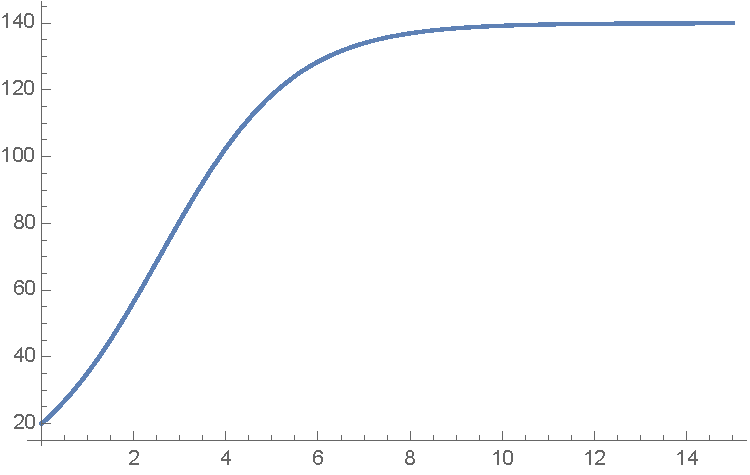
\includegraphics[scale = 0.5]{ex24}
        \caption{Exercise 24}
        \label{fig:ex24}
      \end{figure}


    % \item[29]
    %   \begin{enumerate}[(a)]
    %     \item 
    %       \[
    %         C'(x) = 0.0015x^2 - 0.2x + 12
    %       \]

    %     \item $C'(200) = \$32$. This is approximately the cost to produce one
    %       more item when you are already producing 200 items.

    %     \item The cost of the 201st item is:
    %       \[
    %         C(201) - C(200) \approx \$32.20
    %       \]
    %   \end{enumerate}

    % \item[31]
    %   \begin{enumerate}[(a)]
    %     \item 
    %       \[
    %         A'(x) = \frac{p'(x) - p(x)}{x^2} 
    %       \]

    %       If $A'(x) > 0$, adding more workers increases the average productivity
    %       so the company can make more money.

    %     \item 
    %       \[
    %         A'(x) = \frac{p'(x) - p(x)}{x^2} = \frac{p'(x)}{x^2} - \frac{A(x)}{x} \\
    %       \]

    %       If $p'(x) > A(x) = \frac{p(x)}{x}$, then
    %       \begin{align*}
    %         A'(x) & = \frac{p'(x)}{x^2} - \frac{A(x)}{x} > \frac{A(x)}{x} - \frac{A(x)}{x} = 0 \\
    %         A'(x) & > 0 \\
    %       \end{align*}

    %   \end{enumerate}



    % \item[21]
    %   \begin{enumerate}[(a)]
    %     \item 
    %       \begin{align*}
    %         V             & = \frac{C}{P} \\
    %         \frac{dV}{dP} & = - \frac{C}{P^2} \\
    %       \end{align*}

    %     \item
    %       After 10 minutes, the pressure has increased. The rate of change of
    %       the volume is smaller when the pressure is larger so after 10 minutes
    %       the pressure is increasing at a slower rate.

    %     \item
    %       \begin{align*}
    %         \Beta & = - \frac{1}{V} \cdot \frac{dV}{dP} \\
    %               & = \frac{1}{V} \cdot \cdot \frac{PV}{P} \\
    %               & = \frac{C}{PV} \\
    %       \end{align*}

    %   \end{enumerate}

  \end{description}

  \newpage

  \subsection{Section 3.9}
  \begin{description}
    \item[1]
      \begin{align*}
        V(x)          & = x^3 \\
        \frac{dV}{dt} & = \boxed{ 3x^2 \frac{dx}{dt} } \\
      \end{align*}

    \item[2]
      \begin{enumerate}[(a)]
        \item 
          \begin{align*}
            A(r)          & = \pi r^2 \\
            \frac{dA}{dt} & = \boxed{ 2 \pi r \frac{dr}{dt} } \\
          \end{align*}

        \item 
          \[
            A'(\unit[30]{m}) = 60 \pi \approx \unit[188.5]{m^2/s}
          \]
      \end{enumerate}

    \item[3]
      \begin{align*}
        A(x)          & = x^2 \\
        \frac{dA}{dt} & = 2x \frac{dx}{dt} \\
      \end{align*}

      When the area is $\unit[16]{cm^2}$, the sides are $\unit[4]{cm}$.
      \[
        A'(4) = 2 \cdot 4 \cdot 6 = \boxed{ \unit[48]{cm^2/s} }
      \]

    \newpage

    \item[4]
      \begin{align*}
        A(t)          & = x(t) \cdot y(t) \\
        \frac{dA}{dt} & = \frac{dx}{dt} y(t) + x(t) \cdot \frac{dy}{dt} \\
      \end{align*}

      At the time described:
      \[
        A(t) = \boxed{ \unit[140]{cm^2/s} }
      \]

    \item[5]
      \begin{align*}
        V(t)          & = 25 \pi h(t) \\
        \frac{dV}{dt} & = 25 \pi \frac{dh}{dt} \\
        \\
        3             & = 25 \pi \frac{dh}{dt} \\
        \frac{dh}{dt} & = \boxed{ \unit[\frac{3}{25 \pi}]{m/min} } \\
      \end{align*}

    \item[6]
      \begin{align*}
        V(t)          & = \frac{4}{3} \pi r^3 \\
        \frac{dV}{dt} & = 4 \pi r^2 \frac{dr}{dt} \\
      \end{align*}

      When $\frac{dr}{dt} = \unit[4]{mm/s}$ and $r = \unit[40]{mm}$:
      \[
        \frac{dV}{dt} = \unit[25,600 \pi]{mm^3/s} \approx \boxed{ \unit[80.42]{cm^3/s} }
      \]

    \item[14]
      \begin{align*}
        x(t)          & = 150 - 35 t \\
        \frac{dx}{dt} & = -35 \\
        \\
        y(t)          & = 25 t \\
        \frac{dy}{dt} & = 25 \\
        \\
        r(t)          & = \sqrt{x^2 + y^2} \\
        \frac{dr}{dt} & = \frac{x \frac{dx}{dt} + y \frac{dy}{dt}}{\sqrt{x^2 + y^2}} \\
      \end{align*}

      At 4:00, $\frac{dr}{dt} \approx \boxed{ \unit[21.39]{km/hr} }$

    % \item[15]
    %   Approach one:
    %   \begin{align*}
    %     x(t)          & = 25 t \\
    %     y(t)          & = 60 t \\
    %     r(t)          & = \sqrt{(25t)^2 + (60t)^2} = 65 t \\
    %     \frac{dr}{dt} & = \unit[65]{mi/hr} \\
    %   \end{align*}

    %   The distance is increasing at a constant rate, so it doesn't matter what value you put in for $t$.

    \item[18]
      \begin{enumerate}[(a)]

        \item 
          \begin{align*}
            r(t)          & = \left( 90^2 + x^2 \right) \\
            \frac{dr}{dt} & = \frac{x}{\sqrt{90^2 + x^2}} \frac{dx}{dt} \\
          \end{align*}

          When $x = 45$ and $\frac{dx}{dt} = -24$:
          \[
            \frac{dr}{dt} \approx \boxed{ \unit[-10.73]{ft/s} }
          \]

        \item Since the figure is symmetric, the only thing different for third base at this moment
          is that the distance is increasing instead of decreasing.

      \end{enumerate}

    \item[21]
      \begin{align*}
        x(t) & = 100 \\
        y(t) & = 60t \\
        s(t) & = \frac{xx' + yy'}{\sqrt{x^2 + y^2}} \\
             & = \frac{180t}{\sqrt{9t^2 + 25}}
        \\
        s(4) & = \frac{720}{13} \\
             & \approx \boxed{ \unit[55.38]{km/h} } \\
      \end{align*}

    \item[24]
      The volume is the area of the cross section multiplied by the length. The base of the cross
      section is three times the height of the current water level.

      \begin{align*}
        b(t) & = 3 h(t) \\
        V    & = \frac{1}{2} bh \cdot 10 \\
             & = 5bh \\
             & = 15 h^2 \\
        \\
        \frac{dV}{dt} &= 30 h \frac{dh}{dt} \\
        \frac{dh}{dt} &= \frac{1}{30 h} \cdot \frac{dV}{dt} \\
      \end{align*}

      When $h = \unit[0.5]{ft}$ and $\frac{dV}{dt} = \unit[12]{ft^3/min}$:
      \[
        \frac{dh}{dt} = \boxed{ \unit[0.8]{ft/min} }
      \]

  \end{description}

  \else
    \vspace{10 cm}
    \begin{quote}
      \begin{em}
        Real ``change that you could believe in'' would be an end to empire,
        and an end to wars for corporate greed, not just a change of the shade
        of the political managers.
      \end{em}
    \end{quote}
    \hspace{2 cm} --Mumia Abu-Jamal
  \fi

\end{document}

